\chapter{High-Performance Regimes}\label{ch:HighPerformance}

The development of magnetic-confinement fusion into an economical form of power generation is characterized by two seemingly contrary requirements: first, a high level of energy confinement is necessary to reach the desired level of self-heating of the plasma by fusion products, satisfying triple-product requirements (\cref{eq:tripleproduct}).  At the same time, particle transport must be sufficient to avoid the deleterious effects of accumulated helium ``fusion ash'' and other impurities on fusion performance -- particularly important in the case of the high-$Z$ impurities from the metal plasma-facing walls necessary for reactor-scale devices \cite{Loarte2007}\gnote{more cites?}.

A number of operating scenarios, collectively termed ``high confinement'' or H-modes\cite{Wagner1982}, satisfying these requirements have been developed.  The ``low confinement'' or L-mode operating baseline of energy confinement is characterized through an extensive multi-machine scaling study \cite{Yushmanov1990} by the ITER-89 scaling,

\begin{equation}\label{eq:tau89}
 \tau_{E,ITER89} = 0.048 \times \overline{n}_e^{0.1} M^{0.5} I_p^{0.85} R^{1.2} a^{0.3} \kappa^{0.5} B_T^{0.2} P_{aux}^{-0.5}
\end{equation}

\noindent in which $\overline{n}_e$ is the line-averaged density ($\SI{e20}{\per\meter\cubed}$), $M$ is the atomic mass ($\si{amu}$), $I_p$ is the plasma current ($\si{\mega\ampere}$), $B_T$ is the toroidal field ($\si{T}$), $R$ and $a$ are the major and minor radii in $\si{\meter}$ (see \cref{fig:intro_geometry}), $\kappa$ is the elongation (see \cref{fig:intro_shaping}), and $P_{aux}$ is the externally-applied heating power ($\si{\mega\watt}$).  Compared to this baseline, H-modes represent a significant improvement in performance, with confinement -- here represented in a normalized sense by the $H$-factor, \ie

\begin{equation}\label{eq:H89}
 H_{89} = \frac{\tau_E}{\tau_{E,ITER89}}
\end{equation}

\noindent improved by roughly a factor of two compared to L-mode.\gnote{more specific, cites?}

This improvement in confinement is due to the formation of a \emph{pedestal}, a transport barrier (see \cref{subsec:intro_barriers}) at the edge that greatly slows the transport of particles and/or energy out of the plasma, and accordingly forms a steep-gradient region in density and/or temperature at the edge.  Pedestal formation is achieved through strongly sheared flows in the plasma edge, driven in part by a radial electric field (the ``$E_r$ well'') and the resulting $\vec{E} \times \vec{B}$ flows in the pedestal.  While this flow is difficult to model due to the short scale lengths inherent to the pedestal \cite{Kagan2010,Landreman2012}, the role of edge $E_r$ and flows has been extensively studied both from an experimental \cite{Groebner1990,Burrell1999,Terry2000,McDermott2009a} and a theoretical \cite{Shaing1989,Biglari1990,Kim1991,Ware1996,Burrell1992} standpoint, as has the role of other edge fluctuations coupling into these flows in driving the transition into H-mode \cite{Schmitz2012}.  As the 
pedestal 
structure is known to set a strong constraint on the overall performance in high-confinement regimes \cite{Kinsey2011}, as well as determining the edge stability and heat exhaust properties of the regime, a firm understanding of the pedestal is essential for extrapolation of a high-performance regime to ITER and beyond.

This chapter provides an overview and comparison of different classes of established H-mode operation, particularly regarding their behaviors in the high energy confinement and low particle confinement required for a reactor.  Additionally, observations of Edge-Localized Modes (ELMs) \cite{Zohm1996} are addressed.  We then introduce the access conditions, operation, and global characteristics of \emph{I-mode} -- an alternate high-performance regime with a number of favorable characteristics for reactor operation, and the subject of the balance of this thesis.

\begin{table*}[h]
 \pushtooutside
 \ttabbox{\caption{Typical operating parameters of tokamaks noted in this thesis, along with references to overviews of each machine.  \emph{Note:} all ITER values are projected.\note{check all values here}}\label{tab:tokamaks}}
 {\begin{tabular}{lcccccc}
  \toprule
  \emph{Device} &
  $R/a \;[\si{\meter}]$ &
  %$a \;[\si{\meter}]$ &
  $I_p\;[\si{\mega\ampere}]$ &
  $B_T \;[\si{\tesla}]$ &
  $\overline{n}_e \;[\SI{e19}{\per\meter\cubed}]$ &
  $T_{e0} \;[\si{\kilo\electronvolt}]$ &
%   heating &
  \emph{refs.}
  \\
  \midrule
  C-Mod (USA) &
  $\num{0.67/0.22}$ &
  %$\num{0.22}$ &
  $\le \num{2}$ &
  $3-8.1$ &
  $\le \num{50}$ &
  $\le \num{8}$ &
%   ICRF, LHRF &
  \cite{Hutchinson1994,Greenwald2007,Greenwald2013}
  \\
  DIII-D (USA) &
  $\num{1.67/0.67}$ &
  %$\num{0.67}$ &
  $1-3$ &
  $2.2$ &
  $\num{6}$ &
  $5-10$ &
%   ECRF, NBI &
  \cite{Luxon2002,Luxon2005a,Luxon2005}
  \\
  ASDEX-U (GER) &
  $\num{1.65/0.5}$ &
  %$\num{0.5}$ &
  $\sim 1$ &
  $3.9$ &
  $\num{7.5}$ &
  $2-3$ &
%   &
  \cite{Herrmann2003,Ryter2003,Stroth2013}
  \\
  JET (UK) &
  $\num{3.4/0.9}$ &
  $3-4$ &
  $3.8$ &
  $\num{5}$ &
  $10-20$ &
%   &
  \cite{McDonald2008,Romanelli2013}
  \\
  JT-60U (JAP) &
  $\num{3.4/0.9}$ &
  $3-4$ &
  $4.8$ &
  $\num{5}$ &
  $10-20$ &
%   &
  \cite{Kamada2002,Kitsunezaki2002}
  \\
  JFT-2M (JAP) &
  $\num{1.3/0.35}$ &
  $0.5$ &
  $2.2$ &
  $\num{5}$ &
  $1-2$ &
%   &
  \cite{Kusama2006,Miura2006}
  \\
  ITER* &
  $\num{6.2/2.0}$ &
  $15$ &
  $5.3$ &
  $\num{10}$ &
  $10$ &
%   &
  \cite{Shimada2007,ITER1999,Doyle2007}
  \\
  \bottomrule
 \end{tabular}}
%  {\begin{tabular}{lcccccc}
%   \toprule
%   \emph{Device} &
%   $R/a \;[\si{\meter}]$ &
%   %$a \;[\si{\meter}]$ &
%   $I_p\;[\si{\mega\ampere}]$ &
%   $B_T \;[\si{\tesla}]$ &
%   $\overline{n}_e \;[\SI{e19}{\per\meter\cubed}]$ &
%   $T_{e0} \;[\si{\kilo\electronvolt}]$ &
% %   heating &
%   \emph{refs.}
%   \\
%   \midrule
%   C-Mod &
%   $\num{0.67/0.22}$ &
%   %$\num{0.22}$ &
%   $\le \num{2}$ &
%   $3-8.1$ &
%   $\le \num{50}$ &
%   $\le \num{8}$ &
% %   ICRF, LHRF &
%   \cite{Hutchinson1994,Greenwald2007,Greenwald2013}
%   \\
%   DIII-D &
%   $\num{1.67/0.67}$ &
%   %$\num{0.67}$ &
%   $1-3$ &
%   $2.2$ &
%   $\num{6}$ &
%   $5-10$ &
% %   ECRF, NBI &
%   \cite{Luxon2002,Luxon2005a,Luxon2005}
%   \\
%   ASDEX-U &
%   $\num{1.65/0.5}$ &
%   %$\num{0.5}$ &
%   $\sim 1$ &
%   $3.9$ &
%   $\num{7.5}$ &
%   $2-3$ &
% %   &
%   \cite{Herrmann2003,Ryter2003,Stroth2013}
%   \\
%   JET &
%   $\num{3.4/0.9}$ &
%   $3-4$ &
%   $3.8$ &
%   $\num{5}$ &
%   $10-20$ &
% %   &
%   \cite{McDonald2008,Romanelli2013}
%   \\
%   JT-60U &
%   $\num{3.4/0.9}$ &
%   $3-4$ &
%   $4.8$ &
%   $\num{5}$ &
%   $10-20$ &
% %   &
%   \cite{Kamada2002,Kitsunezaki2002}
%   \\
%   JFT-2M &
%   $\num{1.3/0.35}$ &
%   $0.5$ &
%   $2.2$ &
%   $\num{5}$ &
%   $1-2$ &
% %   &
%   \cite{Kusama2006,Miura2006}
%   \\
%   ITER* &
%   $\num{6.2/2.0}$ &
%   $15$ &
%   $5.3$ &
%   $\num{10}$ &
%   $10$ &
% %   &
%   \cite{Shimada2007,ITER1999}
%   \\
%   \bottomrule
%  \end{tabular}}
\end{table*}

\section{ELM-Free H-Mode}\label{sec:hcr_elmfree}

\begin{figure}[t]
 \pushtooutside
 \fcapside[65mm]{\caption{Characteristic traces of transient ELM-free H-modes, highlighted on the traces (\cref{sec:hcr_elmfree}).  After the L-H transition, density and thermal pressure (and therefore fusion reaction rate and stored energy) rise, while turbulent particle transport is reduced, as seen by the drop in edge $D_\alpha$ light and suppression of turbulence.  However, radiated power rises due to impurity accumulation -- when radiated power reaches a level comparable to total heating power, the plasma drops back into L-mode.}\label{fig:hcr_elmfree}}{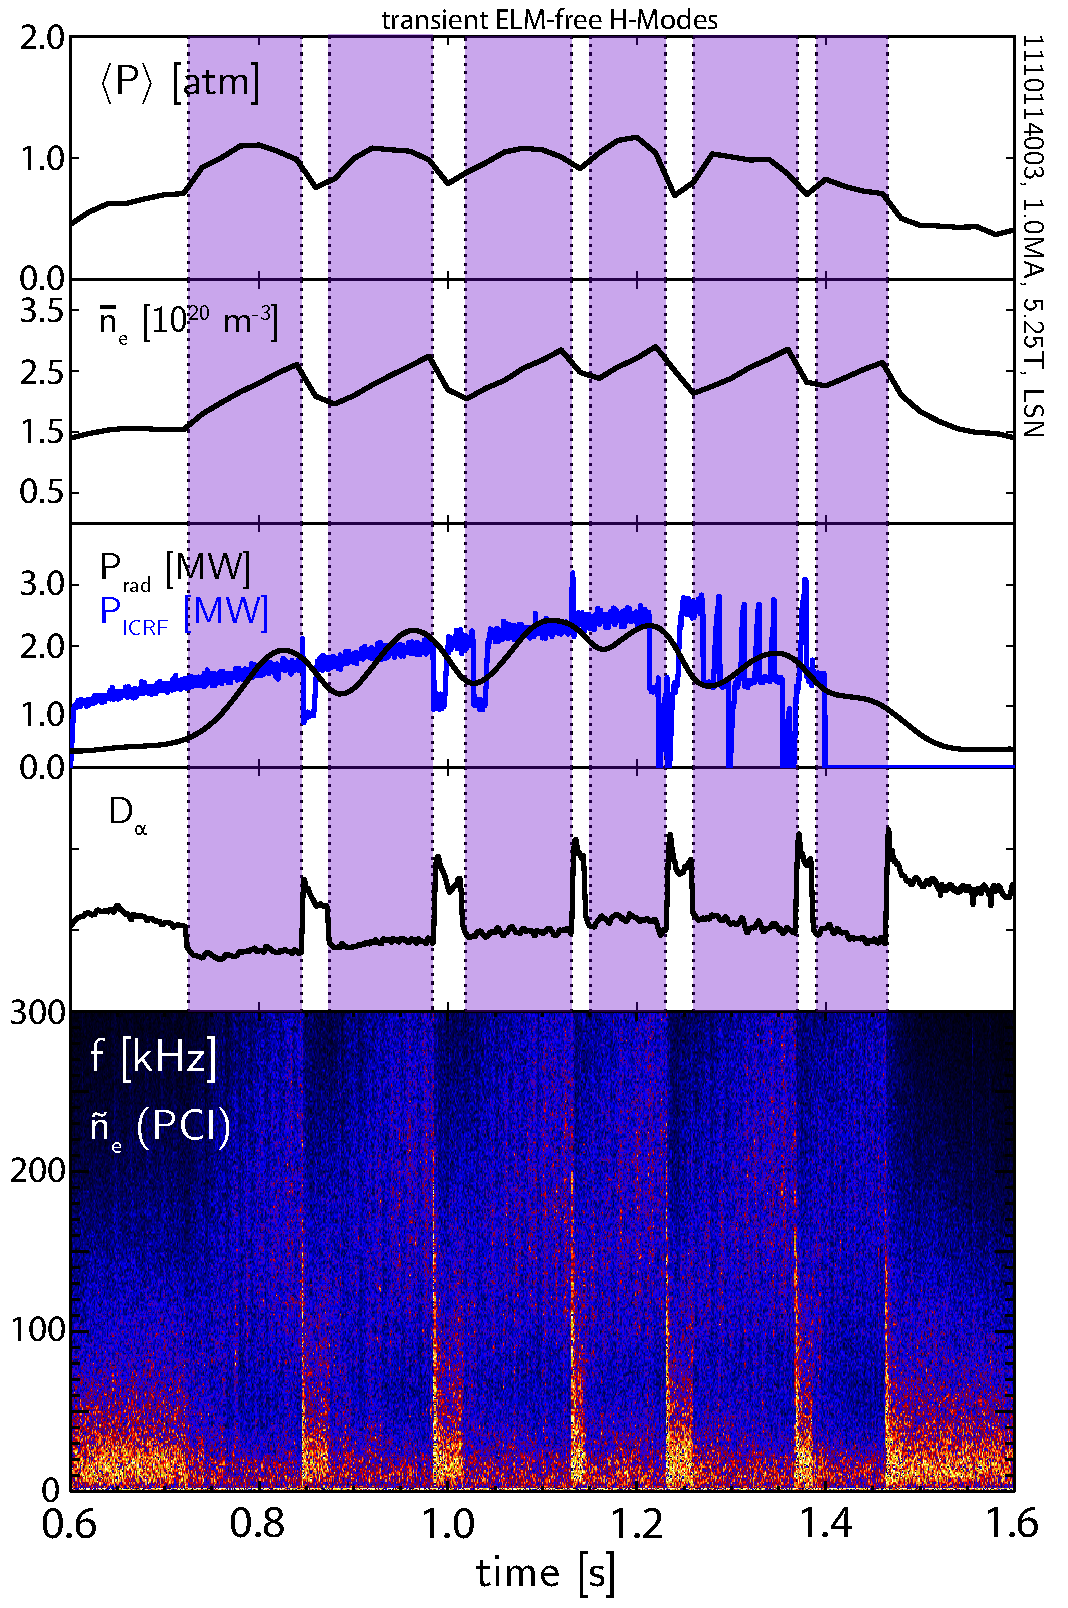
\includegraphics[width=100mm]{graphics/HighPerformanceRegimes/trace_1110114003.pdf}}
\end{figure}

At moderate levels of heating power above the L-H threshold\gnote{cite for $P_{thres}$ here, reword?}, the plasma enters a transient \emph{ELM-free H-mode}, in which an H-mode forms without exhibiting large edge-localized modes (ELMs) \cite{Wagner1982,Keilhacker1984}.  ELM-free H-modes exhibit high levels of both energy and particle confinement, resulting in strong density and temperature pedestals \cite{Hubbard2000,Hatae1998}.  

\nicesectionending

\section{ELMy H-Mode}\label{sec:hcr_elmy}

\subsection{Global Parameters}\label{subsec:hcr_elmy_ped}

\begin{figure}
 \pushtooutside
 \fcapside[65mm]{\caption{Characteristic traces of a steady ELMy H-mode (\cref{sec:hcr_elmy}).  Density and radiated power rise after the L-H transition, but stabilize as the periodic relaxation of the pedestal regulates and flushes impurities from the plasma.  ELM bursts are visible as spikes on the edge $D_\alpha$ signal.}\label{fig:hcr_elmy}}{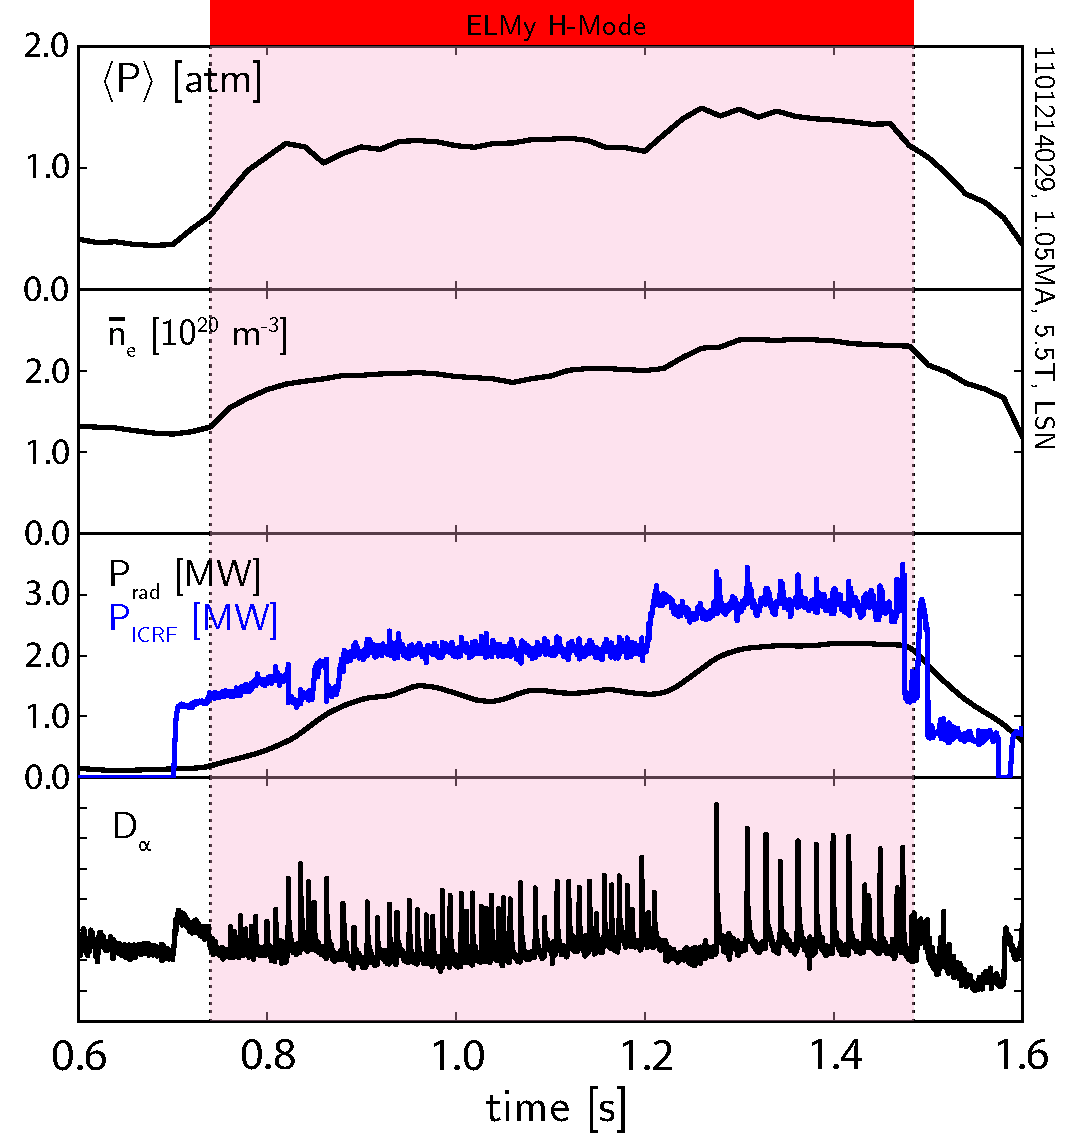
\includegraphics[width=100mm]{graphics/HighPerformanceRegimes/trace_1101214029.pdf}}
\end{figure}

\subsection{Fluctuations and ELMs}\label{subsec:hcr_elmy_fluct}

\subsection{Active ELM Control}\label{subsec:hcr_elmy_control}

\nicesectionending

\section{ELM-Suppressed H-Modes}\label{sec:hcr_elmsuppressed}

In addition to H-modes exhibiting ELMs, classes of H-mode have been established capable of stationary operation with acceptable levels of particle transport (avoiding the radiative collapse and subsequent transient nature found in classical ELM-free H-modes) without exhibiting the bursty heat and particle transport driven by ELMs.  Rather, the pedestal is regulated by a continuous fluctuation localized in the pedestal.  Due to this attractive property, these regimes have been extensively researched\gnote{reword}.  The characteristics of two major types, the Quiescent H-mode (QH-mode) and Enhanced $D_\alpha$ (EDA) H-mode are presented here.

\subsection{QH-Mode}\label{subsec:hcr_qh}

The \emph{Quiescent H-mode} (QH-mode) was first observed on DIII-D \cite{Burrell2002,Groebner2001}, and subsequently achieved on ASDEX Upgrade \cite{Suttrop2003a}, JT-60U \cite{Sakamoto2004}, and JET \cite{Suttrop2005}.  In QH-mode operation, following a brief ELM-free or ELMing phase after the L-H transition, the plasma enters a state with steady averaged density and radiated power, indicating a lack of serious impurity accumulation, despite lacking ELM transport (evident from divertor $D_\alpha$ light, which is ``quiescent'' compared to the characteristic spikes driven by ELMs).  Although QH-mode requires lower densities (average density reduced by roughly a factor of two from comparable ELMy H-modes) with cryopumping for density control, access is otherwise robust, with successful operation across a broad range of shaping, safety factor, current and field \cite{Burrell2002}.  The regime is capable of stationary operation, with the mode sustained for most of the current flat-top on DIII-D ($\sim 25 \tau_E$)
 with very good confinement -- in cases with an internal transport barrier in addition to the pedestal (termed the ``Quiescent Double Barrier'' or QDB regime \cite{Burrell2001,Doyle2001,Greenfield2002}) a confinement metric of $\beta_N H_{89} \sim 7$ was reached (albeit for a briefer period, $\sim 5 \tau_E$), compared to $\beta_N H_{89} \sim 4$ found in ELMy H-modes on DIII-D \cite{Doyle2001}.  Here we use for a normalized pressure metric.\gnote{cite for this?}

\begin{equation}\label{eq:betan}
 \beta_N = \beta \frac{aB_T}{I_p}
\end{equation}

\noindent in $\si{\meter.\tesla\per\mega\ampere}$.  Similarly competitive confinement between QH-mode and ELMy H-mode is seen on ASDEX Upgrade and JET, although the mode on JT-60U is out-performed by ELMy H-mode \cite{Oyama2006}.  The pedestal density is reduced (comparable to the reduction in globally-averaged density) in QH-mode compared to ELMy H-mode, and excess fueling to the edge by gas puffing, pellet fueling, or wall outgassing destroys the QH-mode.  However, pedestal temperatures are typically somewhat higher \cite{Doyle2001}, thus the mode is found at ITER-relevant low collisionalities.  Pedestal pressure gradients are comparable to those found in ELMy H-mode, implying stabilization of the peeling-ballooning MHD modes typically associated with the ELM trigger \cite{Burrell2002}.\gnote{elaborate?}  A particularly strong $E_r$ well ($2-3$ times deeper than in comparable ELMy H-modes) is also observed in the QH-mode pedestal \cite{Greenfield2002}.

In place of bursty ELM transport, the pedestal in QH-mode is continuously regulated by the \emph{Edge Harmonic Oscillation} (EHO), an MHD mode observed in density, temperature, and magnetic fluctuations \cite{Burrell2002}.  The EHO is made up of distinct harmonics with toroidal mode numbers $n \sim 1-10$; these harmonics are directly observed in the particle flux at the divertor, indicating that the EHO is responsible for density regulation in QH-mode \cite{Doyle2001}.  MHD modeling approaches similar to that described in \cref{ch:Modeling} indicate that the EHO is a saturated peeling mode \cite{Snyder2007,Osborne2008,Snyder2012}.  This is consistent with the low pedestal collisionality in the QH-mode pedestal (lower collisionalities and higher bootstrap currents tends to drive the pedestal towards the peeling side of the peeling-ballooning MHD boundary, as described in \cref{ch:Modeling}), and with the observed localization of the EHO in the region of strongest $E_r$ and rotation shear \cite{Burrell2001}.  
the saturated mode is driven by the strong rotation shear in the edge -- while this typically destabilizes low-$n$ MHD modes\gnote{pull ref 9 from Burrell2009?}, in the case of the EHO the magnetic component of the mode couples to the vacuum-vessel wall as the rotation spins up, providing the drag force necessary to saturate the mode at finite amplitude \cite{Burrell2009}.  This maintains the pedestal below the current-driven peeling boundary associated with the ELM trigger, providing the ELM suppression in QH-mode \cite{Snyder2012}.

Historically, QH-mode operation has required significant neutral-beam inputs directed counter the plasma current direction, providing the necessary rotation \cite{Burrell2002}.  However, counter-current beam operation drives significant fast-ion losses into the outer wall, necessitating operation with a large outer gap to avoid wall outgassing.  More recent experiments have successfully generated QH-modes with co-current beam injection \cite{Burrell2009} and with torque from non-axisymmetric magnetic fields \cite{Garofalo2011,Burrell2013}.  The latter is of particular importance, as it is not expected that the NBI systems on ITER will drive sufficient torque to produce QH-mode \cite{Garofalo2011}.  In addition to the requirement for externally-supplied torque to maintain the mode, QH-mode suffers from accumulation of high-$Z$ impurities -- while lower-$Z$ ions are flushed from the plasma by the EHO, high-$Z$ impurities tend to accumulate in the core \cite{Doyle2001,Suttrop2005}, which may present 
difficulties attaining QH-mode on metal-walled machines where high-$Z$ impurities dominate.  Nevertheless QH-mode is an attractive option for a reactor regime.

\subsection{EDA H-Mode}\label{subsec:hcr_eda}

\begin{figure}
 \pushtooutside
 \fcapside[65mm]{\caption{Characteristic traces of an EDA H-mode on C-Mod (\cref{subsec:hcr_eda}).  Following a brief ELM-free phase, the plasma density and radiated power stabilizes at a sustainable level.  The edge transport barrier is regulated by the continuous QCM fluctuation rather than bursty ELM transport.}\label{fig:hcr_eda}}{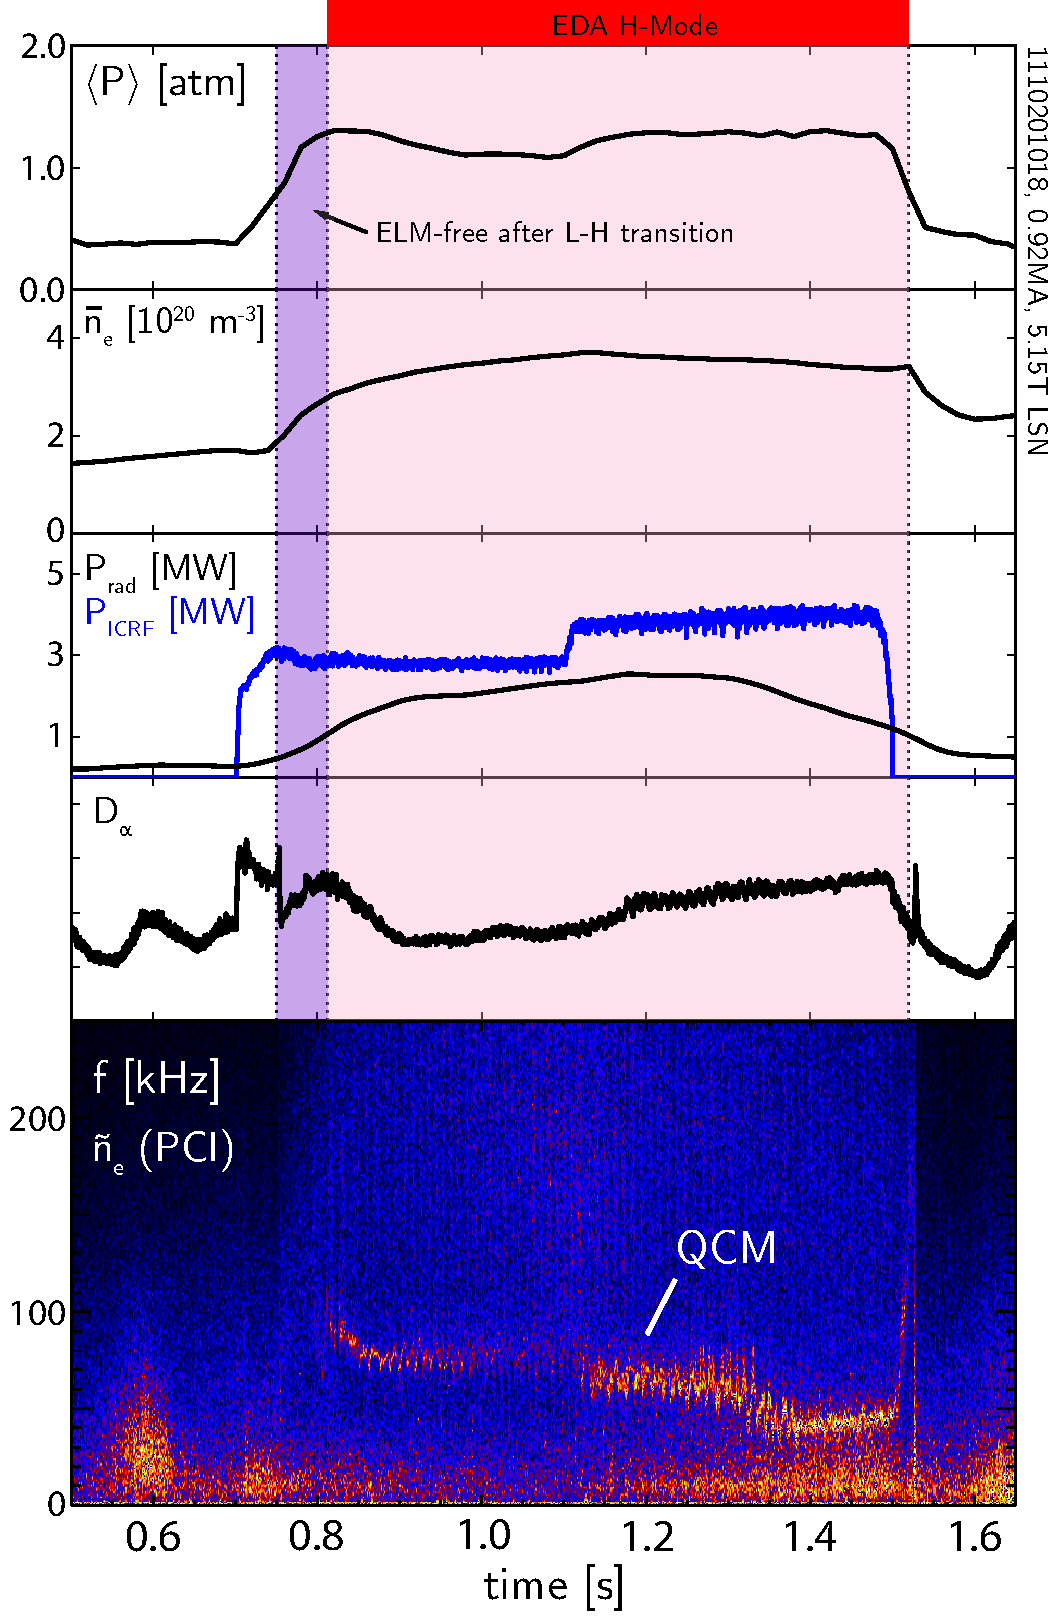
\includegraphics[width=100mm]{graphics/HighPerformanceRegimes/trace_1110201018.pdf}}
\end{figure}

The \emph{Enhanced $D_\alpha$ H-mode} (EDA H-mode) is a high-performance regime explored on the Alcator C-Mod tokamak \cite{Greenwald1999,Hubbard2001,Hughes2005}\gnote{time trace, fluctuations, profile comparison between EDA, ELMy}.  Along with transient ELM-free H-modes, the EDA regime is the customary approach to H-mode operation on C-Mod, unlike other major tokamak experiments; the Type-I ELMy H-mode typical on other devices requires an abnormal shaping to more easily reach the stability boundary associated with the ELM trigger on C-Mod \cite{Hughes2013}\gnote{make sure to elaborate on this in ELMy section or reference later}.  In EDA operation, the L-H transition is followed by a rise in radiated power and density similar to an ELM-free H-mode.  However, shortly thereafter the H-mode stabilizes at steady density \cite{Greenwald1999}, with the radiated power held at $P_{rad}/P_{in} \sim 30\%$ \cite{Hubbard1998}, allowing steady operation (maintained for most of the steady current phase, $\sim 10\tau_E$) 
and good performance, with $H_{89} \sim 1.9$, $H_{98} \sim 1$ \cite{Hubbard2001}.  Notably, modeling of the pedestal in EDA H-mode indicates energy confinement with potentially weaker degradation of $\tau_E$ with input heating power \cite{Hughes2002,Hughes2005,Hughes2006}\gnote{move this elsewhere?}.  Rather than bursty ELM transport, the EDA pedestal is regulated by a continuous density pumpout, with divertor $D_\alpha$ signals (indicative of the density exhaust from the plasma) recovering to near L-mode levels after an initial drop at the L-H transition\gnote{check this, reword?}.  Access to EDA H-mode is fairly robust, although it is strongly favored by higher collisionality ($\nu^* > 1$) and edge safety factor \cite{Hughes2002,Mossessian2002} and by strong shaping \cite{Mossessian2002}\gnote{define $\nu^*$ here, or earlier?}.  Although a higher collisionality is observed to be required at lower values of $q_{95}$, a collisionality threshold alone is insufficient to explain EDA access \cite{Hughes2002}.  
Instead, EDA and ELM-free H-modes are separated in a phase space of collisionality and normalized pressure gradient ($\nu^*$-$\alpha_{MHD}$)\gnote{define $\alpha_{MHD}$ before here} -- however, the transition between the two regimes is soft, with the EDA smoothly appearing at higher pressure gradients and collisionalities rather than exhibiting a sharp transition \cite{Hughes2007a}.

While the pedestal pressure in EDA H-mode is comparable to that in ELMy H-mode, the pedestal profiles in EDA tend towards higher density and lower temperature -- this strongly alters the collisionality (consistent with the observed requirements for $\nu^* > 1$ for EDA access) and bootstrap current near the edge, with significant impact on MHD behavior.  The pedestal appears to be limited by transport effects rather than stability -- the pedestal is modeled to be stable to ideal MHD effects \cite{Mossessian2002,Hughes2013}, despite exhibiting a $\nabla p \sim I_p^2$ trend expected from a ballooning instability \cite{Hughes2006}\gnote{elaborate here, or elsewhere?}.  Instead, the pedestal density is determined by the interplay between an inward particle pinch and outward density transport.  Outward particle transport is decreases at higher currents (and therefore higher densities at fixed Greenwald fraction\gnote{explain or reword}), while the high pedestal density results in strong ionization in the scrape-
off layer and an edge that is relatively opaque to neutrals \cite{Hubbard2007,Greenwald2007}.  As a result, the density will rise until the transport saturates -- additional fueling through the edge triggers minimal response, while a density drop is countered by increased particle particle confinement to recover the density, resulting in pedestal and global density values set by the plasma current, with weak dependence on other engineering parameters \cite{Hughes2007}.

The regulation of the pedestal in EDA H-mode is provided by the \emph{Quasi-Coherent Mode} (QCM), a field-aligned electromagnetic fluctuation localized in the steep-gradient region of the pedestal \cite{Hubbard2001,Terry2005,Mossessian2003}.  The QCM is a fairly narrow-band ($\delta f/f \sim 10\%$) mode strongly visible in density and magnetic fluctuations, with a centroid frequency of $50-200\;\si{\kilo\hertz}$ and a fairly short poloidal wavelength, $k_\theta \sim \SI{1.5}{\per\centi\meter}$ \cite{Terry2005}.  QCM fluctuations are visible in the density flux to the divertor, indicating that the QCM fluctuation is directly responsible for the particle transport through the EDA H-mode pedestal \cite{Greenwald2007,Terry2005}.  Numerical modeling of the EDA H-mode pedestal suggests a resistive ballooning mode (the collisional analogue to the ideal ballooning MHD mode found in ELMy H-modes\gnote{describe this in ELMy section}) for the QCM \cite{Mazurenko2002,Hughes2007a}.  This is consistent with experimental 
observations of the EDA pedestal -- the requirement of high collisionality (the QCM dissappears below $\nu^* \sim 0.1$) suggests a resistive effect \cite{Hughes2013}, while the favored high edge pressure gradient ($\alpha_{MHD}$) suggests a ballooning instability.  At high power and high edge pressure gradient, the QCM is replaced by small, high-frequency ELMs \cite{Mossessian2002,Mossessian2003,Hughes2007a}, potentially indicating that the pedestal is ``burning through'' the resistive-ballooning regulation of the pedestal and reaching the ideal MHD boundary associated with the ELM trigger.\gnote{ref here about high collisionality in other small-ELM regimes?}

The EDA H-mode presents another potential route to reactor-scale operation with naturally-suppressed large ELMs.  The regime is robustly accessible on C-Mod using only RF heating with no external momentum sources or non-axisymmetric magnetic coils, with good confinement and acceptable levels of impurity accumulation and radiated power consistent with high performance \cite{Hughes2011}.  Moreover, there is an extensive body of research studying the EDA H-mode on a machine with all-metal walls, with ITER-relevant heat flux and edge neutral behavior \cite{Hubbard2007,Greenwald2007}, and with similar electron-ion equilibration to that expected for ITER \cite{McDermott2009a}.  However, the necessary collisionality ($\nu^* > 1$) for the QCM fluctuation is significantly higher than the expected levels for the ITER pedestal ($\nu^* < 0.1$), inconsistent with unaided access to the EDA regime\gnote{where to go with this, mention shoelace?}.\nicesectionending

\section{I-Mode}\label{sec:hcr_imode}

\subsection{Access and Operation}\label{subsec:hcr_imode_access}

\subsection{Global Performance}\label{subsec:hcr_imode_performance}

\subsection{Edge Fluctuations -- the Weakly-Coherent Mode}\label{subsec:hcr_imode_wcm}

\nicechapterending

\bibliographystyle{../plainurl}
\bibliography{../references}